\documentclass[a4paper, article, english, oneside, unknownkeysallowed, 12pt]{memoir} 
\usepackage{preamble}


\usepackage[
backend=biber,
style=authoryear-ibid,
maxcitenames=2, % show up to 2 authors in citations
mincitenames=1, % use "et al." if more than 2
maxbibnames=10, % show up to 10 names in bibliography
minbibnames=1,
uniquelist=false,
uniquename=false
]{biblatex}


\addbibresource{causal_effect_schools.bib}

\AtEveryBibitem{%
  \clearfield{urlyear}%
  \clearfield{urlmonth}%
  \clearfield{urlday}%
  \clearfield{urldate}%
}

% Name and Title
\title{Do High Schools Shape College Choices? Evidence from Centralized Assignment in Chile}
\author{Anonymous}
\date{July 2026}

% Header (top) and footer (bottom)
\pagestyle{fancy}
\fancyhead[R]{\emph{Do High Schools Shape College Choices?}}
 \fancyhead[L]{}
\fancyfoot[R]{}
\fancyfoot[L]{}


\begin{document}

% Prints title block from macros given above
\maketitle

\begin{abstract}
School quality is usually measured with test scores, but high schools may also shape students' college choices.
This paper studies this question in Chile, where centralized assignment creates lottery variation in high-school offers.
I link assignment records to administrative data on school enrollment, standardized achievement, and higher-education applications and enrollment.
I estimate observational school value added for math, verbal achievement, enrollment in high-premium institutions and high-premium fields, and projected program income, using a rich set of pre-treatment controls.
I then test whether lottery-induced attendance at higher-value-added schools improves the corresponding outcome, controlling for expected value added in each student's assignment portfolio.
Achievement forecast coefficient estimates are 0.884 for math and 0.885 for verbal achievement, close to benchmarks from settings with lagged test scores.
Higher-education value added also predicts causal changes in later choices: pass-through is 0.497 for high-premium-institution enrollment, 0.803 for high-premium-field enrollment, and 0.311 for log projected program income.
Heterogeneity estimates suggest that the pass-through of math value added varies across the baseline math achievement distribution.
Gender also reveals important heterogeneity in achievement pass-through, with value added more informative for girls.
Lastly, an ordered value-added horse race shows that projected-income gains are not primarily summarized by math value added, but rather by other dimensions of value added.
High schools therefore shape college choices through dimensions of school value that achievement value added alone does not capture.
Choices that appear to reveal student preferences may thus partly reflect the information, expectations, and preparation produced by the high school attended.
\end{abstract}

% Prints a table of contents
\setcounter{tocdepth}{2}
\renewcommand\contentsname{}
%\tableofcontents* 

\clearpage
\section{Introduction}

School quality is usually summarized by achievement.
This is natural: test scores are widely available, comparable across schools, and even predictive of later outcomes. \parencite{chetty_how_2011}
But school and teacher effects are not necessarily one-dimensional.
Recent work shows that schools and teachers can affect attendance, behavior, crime, teenage motherhood, labor-market outcomes, and other long-run outcomes in ways that are only weakly related to test-score effects \parencite{jackson_what_2018, beuermann_what_2023, rose_effects_2022, angrist_methods_2023}.
Families and policymakers might therefore care about school quality measures that capture more than just achievement.

This broader view of school quality is especially relevant for high schools.
High schools are the last formal educational institutions students attend before making higher-education choices, and those choices are immensely consequential.
Whether students enter higher education, which institutions they attend, and which fields they choose all matter because returns vary substantially across institutions and, especially, fields of study \parencite{kirkeboen_field_2016}.
Yet many measures of school effects on higher education are coarse, focusing on indicators for enrollment or persistence rather than on the type of institution or field students enter.

There are also good reasons to think that higher-education choices are shaped by frictions that schools may influence.
Prior work documents large differences in application and enrollment behavior across groups of students, and shows that relatively small interventions can change college search, application behavior, and major choice \parencite{hoxby_what_2015, dynarski_closing_2021, hastings_informed_2016, chetty_diversifying_2025}.
If high schools differ in counseling, information provision, expectations, peer norms, academic confidence, or preparation for particular fields, then their effects on higher education may extend beyond their effects on achievement.

This possibility also changes how higher-education choices should be interpreted.
Decisions not to continue to higher education, to avoid particular fields, or to attend lower-quality institutions are often viewed as revealing stable preferences or privately optimal responses to expected returns.
Yet expected returns and the options students perceive may themselves depend on the information, preparation, and support provided by their high school.
A choice can therefore be privately optimal given beliefs and preparation that the school helped produce, while still being causally affected by the school attended.
This distinction is especially relevant in settings where families have limited information about educational options and access to counseling varies across schools.

This paper asks whether high schools causally affect higher-education choices, and whether those effects are captured by traditional achievement value added.
The main empirical challenge arises from the fact that students and families sort across schools.
Families choose schools based on resources, preferences, networks, location, and expectations; these same characteristics may also shape later higher-education choices.
As a result, differences across schools may reflect both causal school effects and the underlying characteristics of the students and families who select into them.

I address this challenge using Chile's centralized school assignment system, the Sistema de Admisi\'on Escolar (SAE).
SAE assigns students to public and private-subsidized schools through a centralized mechanism that uses random tie-breakers when schools are oversubscribed.
The system covers a large national school sector, allowing me to study school effects at a scale that is unusual in lottery-based designs.
This assignment variation can be linked to administrative data covering school enrollment, standardized tests, and higher-education applications and enrollment.
Linking random assignment in the mechanism to higher-education choices allows me to answer this question in a national context.


The analysis proceeds in two steps.
First, I estimate observational value added for each school and outcome in the broad panel.
These measures are school fixed effects from regressions that adjust for rich pre-treatment controls, including grade-4 standardized test scores, family-background variables, and middle-school controls.
Second, I use SAE lottery offers to ask whether schools that look better in observational value-added terms also produce larger causal effects, while controlling for expected value added in each student's assignment portfolio.


I summarize this relationship with a forecast coefficient, $\theta$ in line with \textcite{angrist_leveraging_2017}\footnote{I refer to the forecast coefficient as pass-through interchangeably}.
If $\theta=1$, then the causal effect induced by complying with a lottery offer equals the gain predicted by observational value added for that outcome.
If $\theta=0$, the observational value-added measure has no causal predictive content along the lottery-induced margin.
The main estimates suggest meaningful pass-through.
For achievement, the estimates are 0.884 for math and 0.885 for verbal achievement.
For higher-education choices, the forecast coefficients are 0.497 for enrollment in a high-premium institution, 0.803 for enrollment in a high-premium field, and 0.311 for log projected program income.
In practical terms, schools that observationally look better at raising achievement or higher-education outcomes also predict causal effects on those same outcomes, though the causal effects are smaller than the value-added might suggest.
%The achievement estimates are close to comparable validation estimates in \textcite{angrist_leveraging_2017} despite the absence of immediately lagged outcomes.
%This validates the rich set of pre-treatment controls used here, which can also be applied to outcomes, such as higher-education choices, for which lagged measures are unavailable.

I then ask for whom observational value-added measures are most informative.
Splitting the sample by baseline grade-4 math achievement shows that, relative to students in the middle quintile, math value added is substantially less predictive in the bottom quintile and marginally more predictive in the top quintile.
Math and verbal achievement also show statistically significant differences by gender: achievement value-added measures are less informative for boys.
These results point to meaningful heterogeneity in achievement, yet remarkable stability for the other higher-education dimensions.

Finally, I examine which dimensions of school value added best predict gains in projected program income, a proxy for later earnings.
For interpretation, I use an ordered horse race: math value added enters first, high-premium-institution value added enters after removing its school-level association with math, and high-premium-field value added enters after removing its association with the first two dimensions.
In this specification, the incremental high-premium-field dimension remains positive and precisely estimated, while math value added does not carry the projected-income signal once the higher-education choice dimensions are included.
These results are difficult to reconcile with a view in which math achievement fully summarizes the school dimensions relevant for projected income.

The paper contributes to three literatures.
First, it contributes to work on teacher and school value added.
A large literature estimates the effects of teachers and schools on test scores and longer-run outcomes \parencite{chetty_measuring_2014, dobbie_medium-term_2015, jackson_what_2018, beuermann_what_2023, rose_effects_2022}.
This work increasingly emphasizes that test-score value added may miss important dimensions of educational production.
I extend this idea to high-school effects on higher-education choices, focusing not only on enrollment or achievement but also on whether students enter high-premium fields, high-premium institutions, and programs with higher projected earnings.


Second, the paper contributes to the literature using lotteries and centralized assignment systems to estimate school effects \parencite{abdulkadiroglu_elite_2014, abdulkadiroglu_research_2017, angrist_credible_2024}.
In the spirit of \textcite{angrist_leveraging_2017}, I ask whether observational value-added measures are useful guides to causal school effects.
The contribution here is to apply this pass-through logic to a national high-school assignment system and to outcomes observed after students transition into higher education.

Third, the paper contributes to work on higher-education choice.
Prior research shows that the field and institution students choose matter for later outcomes, and that information and application frictions can change those choices \parencite{kirkeboen_field_2016, hoxby_what_2015, dynarski_closing_2021, hastings_informed_2016, chetty_diversifying_2025}.
I study high schools as a possible upstream source of these differences.
Rather than evaluating a particular counseling or information intervention, the paper measures whether the high-school system itself generates causal differences in students' higher-education paths.

The rest of the paper is organized as follows.
Section 2 describes the Chilean setting and the linked administrative data.
Section 3 presents the empirical framework.
Section 4 reports the main results, heterogeneity by baseline achievement and gender, and the ordered value-added horse race for projected program income.
Section 5 concludes.

\clearpage
\section{Context and Data}

\subsection{Institutional Setting}

Chile is a useful setting for this project because national administrative data records school enrollment, academic histories, standardized achievement, and higher-education choices with scrambled individual identifiers that allow students to be matched across systems.
Formal secondary education begins in grade 9 and lasts four years.
Students may attend public, private-subsidized, or private non-subsidized schools.
Public and private-subsidized schools are publicly financed and participate in the centralized school assignment system described below, while private non-subsidized schools remain outside that mechanism.
In the broad grade-8 universe used in the analysis, private non-subsidized schools account for about 9.3\% of students.
The lottery-based analysis is therefore drawn from the public and private-subsidized sector, with additional sample restrictions for timely SAE application and assignment risk described below.

\subsection{Student Panel and Baseline Controls}

I construct the broad analysis panel by merging annual enrollment, grade progression, attendance, grades, and completion records using the scrambled student identifier.
The linked administrative panel starts from the universe of students first observed in grade 8 between 2017 and 2021, producing 1,197,982 students across five cohorts.
I define each student's cohort by the year of grade-8 enrollment. 

For the principal value-added sample, I then retain the 2017--2020 cohorts, leaving 944,510 students across four cohorts.
I make this cohort restriction because these cohorts have comparable grade-4 SIMCE baseline controls; the 2021 cohort does not.
The main high-school exposure is observed for 4,133 schools with a unique identifier (RBD).
I define high-school exposure as the school identifier where a student spends the most time after grade 8.
This definition smooths over short enrollment spells and transfers, and it gives a single high-school measure for each student.
I define middle-school attendance analogously as the RBD where the student spends the most time in grades 5 to 8.
The same histories let me construct pre-treatment middle-school controls, including standardized measures of grades and attendance before high school.

Baseline achievement comes from SIMCE, Chile's national standardized assessment system.
SIMCE is administered in different grades depending on the year. 
This always includes grade 4 and occasionally grades 8 and 10.
Unfortunately grade-8 and grade-10 measures are not available for all the studied cohorts.
I therefore use grade-4 SIMCE as the main pre-treatment achievement control.
Among the 2017--2020 value-added cohorts, both grade-4 SIMCE math and language are observed for 772,083 students in the raw panel and for 769,659 students after requiring a valid high-school exposure and age range.
The final controlled value-added sample contains 757,999 students after adding the remaining baseline and middle-school controls.

The SIMCE files also contain parent-survey information.
I use these surveys to measure family background before treatment, including household income, parental education, indigenous origin of the parents, and early-childhood attendance.
These variables are useful because they proxy for family resources and prior investments that may influence both high-school choices and later higher-education outcomes.
When parent-survey variables are missing, I use middle school and neighborhood cells to impute medians where enough donor observations are available; remaining missing values are left missing.

\begin{table}[H]
\centering
\caption{Main data sources and sample sizes}
\label{tab:data-samples}
\begin{tabular}{lr}
\toprule
Sample definition & Students \\
\midrule
Linked grade-8 universe, 2017--2021 & 1,197,982 \\
\midrule 
Cohorts 2017--2020 & 944,510 \\
+ valid high-school RBD and age 12--16 & 931,547 \\
+ complete value-added control set & 757,999 \\
+ math or verbal admission-test outcome & 571,110 \\
\midrule
Cohorts 2018--2021 & 959,514 \\
+ timely SAE & 409,737 \\
+ assignment risk & 226,195 \\
+ complete lottery control set & 139,317 \\
+ math or verbal admission-test outcome & 95,705 \\
\bottomrule
\end{tabular}
\end{table}

Table~\ref{tab:data-samples} summarizes how the linked administrative sources map into the two samples used in the analysis.
Rows in the value-added panel should be read cumulatively after restricting to the principal 2017--2020 cohorts.
The broad complete-control panel is used to estimate the main school value-added measures, while the SAE lottery exam-taker sample is used to validate score-based value-added measures using assignment variation.

\subsection{Centralized School Assignment}

Chile's centralized school assignment system, the Sistema de Admisi\'on Escolar (SAE), assigns students to participating schools through a version of student-proposing Deferred Acceptance.
Families submit ranked lists of schools.
The mechanism combines these rankings with school vacancies and priority rules, and it uses random tie-breakers when there are more applicants than seats within a priority group.
Conditional on the information that determines priorities and assignment probabilities, these tie-breakers generate the quasi-experimental variation used in the empirical design, following the centralized-assignment research design described by \textcite{abdulkadiroglu_research_2017}.
SAE started in 2017 in some regions and was rolled out nationally in 2018. 
I use applications to grade-9 vacancies starting in 2018 to construct the lottery sample.


Implementing this design requires recovering each applicant's probability of assignment to each school in the submitted portfolio.
I do this by replicating the SAE assignment algorithm and repeatedly simulating counterfactual lottery draws.
As a diagnostic check, when I run the replicated algorithm using the original lottery numbers for the 2018--2021 regular grade-9 processes, I reproduce more than 99\% of observed first-round assignments in each of the four cohorts.
The remaining mismatch reflects institutional features that are difficult to fully recover from public documentation, but the high replication rate gives confidence that the simulated probabilities capture the relevant assignment risk.

The estimation sample consists of timely SAE applicants: students who apply in the assignment process corresponding to their grade-8 cohort and who have assignment risk in the simulated data.
Assignment risk means that the simulated assignment probabilities do not place all probability mass on a single school.

As shown in Table~\ref{tab:data-samples}, the lottery sample contains 226,195 students with assignment risk across the 2018--2021 cohorts.
The complete lottery-control set contains 139,317 students. Grade-4 SIMCE baseline controls are not broadly available for the 2021 cohort, so only 3,203 students from that cohort remain at this stage.
The score-based estimation sample further restricts to the 95,705 lottery-risk students with an observed math or verbal national admission-test score.
On average, these students have positive simulated assignment probability at about 3.1 schools; the median is 3 and the 90th percentile is 5.

%Among applicants with assignment risk, 85.4\% receive a first-round SAE offer.
%The remaining 14.6\% have no first-round assignment (\texttt{rbd\_admitido}) in the regular-process results; they are retained, with their first-round offer value set to zero.
%The first-round offered RBD is the source of lottery variation, while the student's realized high-school exposure is measured by the most-time RBD described above.

The value-added exercise uses the broader complete-control panel, while the causal estimates use the smaller lottery-risk sample.
This distinction is central to the interpretation.
The broad panel improves precision in estimating school-level outcome gradients, and the lottery sample then tests whether those observational value-added measures have causal signal on the centralized-assignment margin.
The results therefore speak most directly to students and schools represented in the SAE lottery-risk sample.
Because SAE covers the public and private-subsidized sector, this is a large and policy-relevant part of the high-school market, but extrapolating to private non-subsidized schools or non-lottery margins requires assuming that the same value-added gradients are comparable there.

\subsection{Higher-Education Outcomes}

The higher-education system also generates administrative data on applications, admission scores, and enrollment.
Taking the national admission exam is a choice for secondary-school students, but it is the standard route into selective higher education.
Students who apply through the centralized admission system take mandatory math and verbal components, and may also take optional subject exams.\footnote{The national admission exam was called the PSU through 2020, the PTU in 2021--2022, and the PAES from 2023 onward.}
I use the mandatory math and verbal scores as achievement outcomes, standardizing them within test year to make them comparable across test regimes.

Higher-education applications and admissions are organized at the program-institution level.
A student's admission depends on entrance-exam scores, school GPA-based scores, ranked program preferences, and the weights each program assigns to score components.
This structure is useful because it makes higher-education choices much richer than a single college-enrollment indicator: students choose not only whether to enroll, but also which institution, program, and field to pursue.

Students in the sample have not yet finished higher education, so I cannot observe their realized earnings. 
I take advantage of MiFuturo, an information source run by the Ministry of Education that reports labor-market statistics at the program level.
I use its reported average income in the fourth year after graduation to assign an earnings proxy to higher-education options. 

Because the MiFuturo income file is not observed at the exact enrollment-program code used in the matricula records, I do not treat it as a direct one-to-one match for every student-program record.
Instead, I estimate log-income fixed-effect models in the MiFuturo data using institution and generic-program cells.
Figure~\ref{fig:mifuturo-field-income-premia} shows the estimated generic-program fixed effects organized by field.
I then use generic-program and institution estimates to construct projected-income measures for the matriculated programs observed in the student panel when the exact program has no direct MiFuturo value.

\begin{figure}[!htbp]
\centering
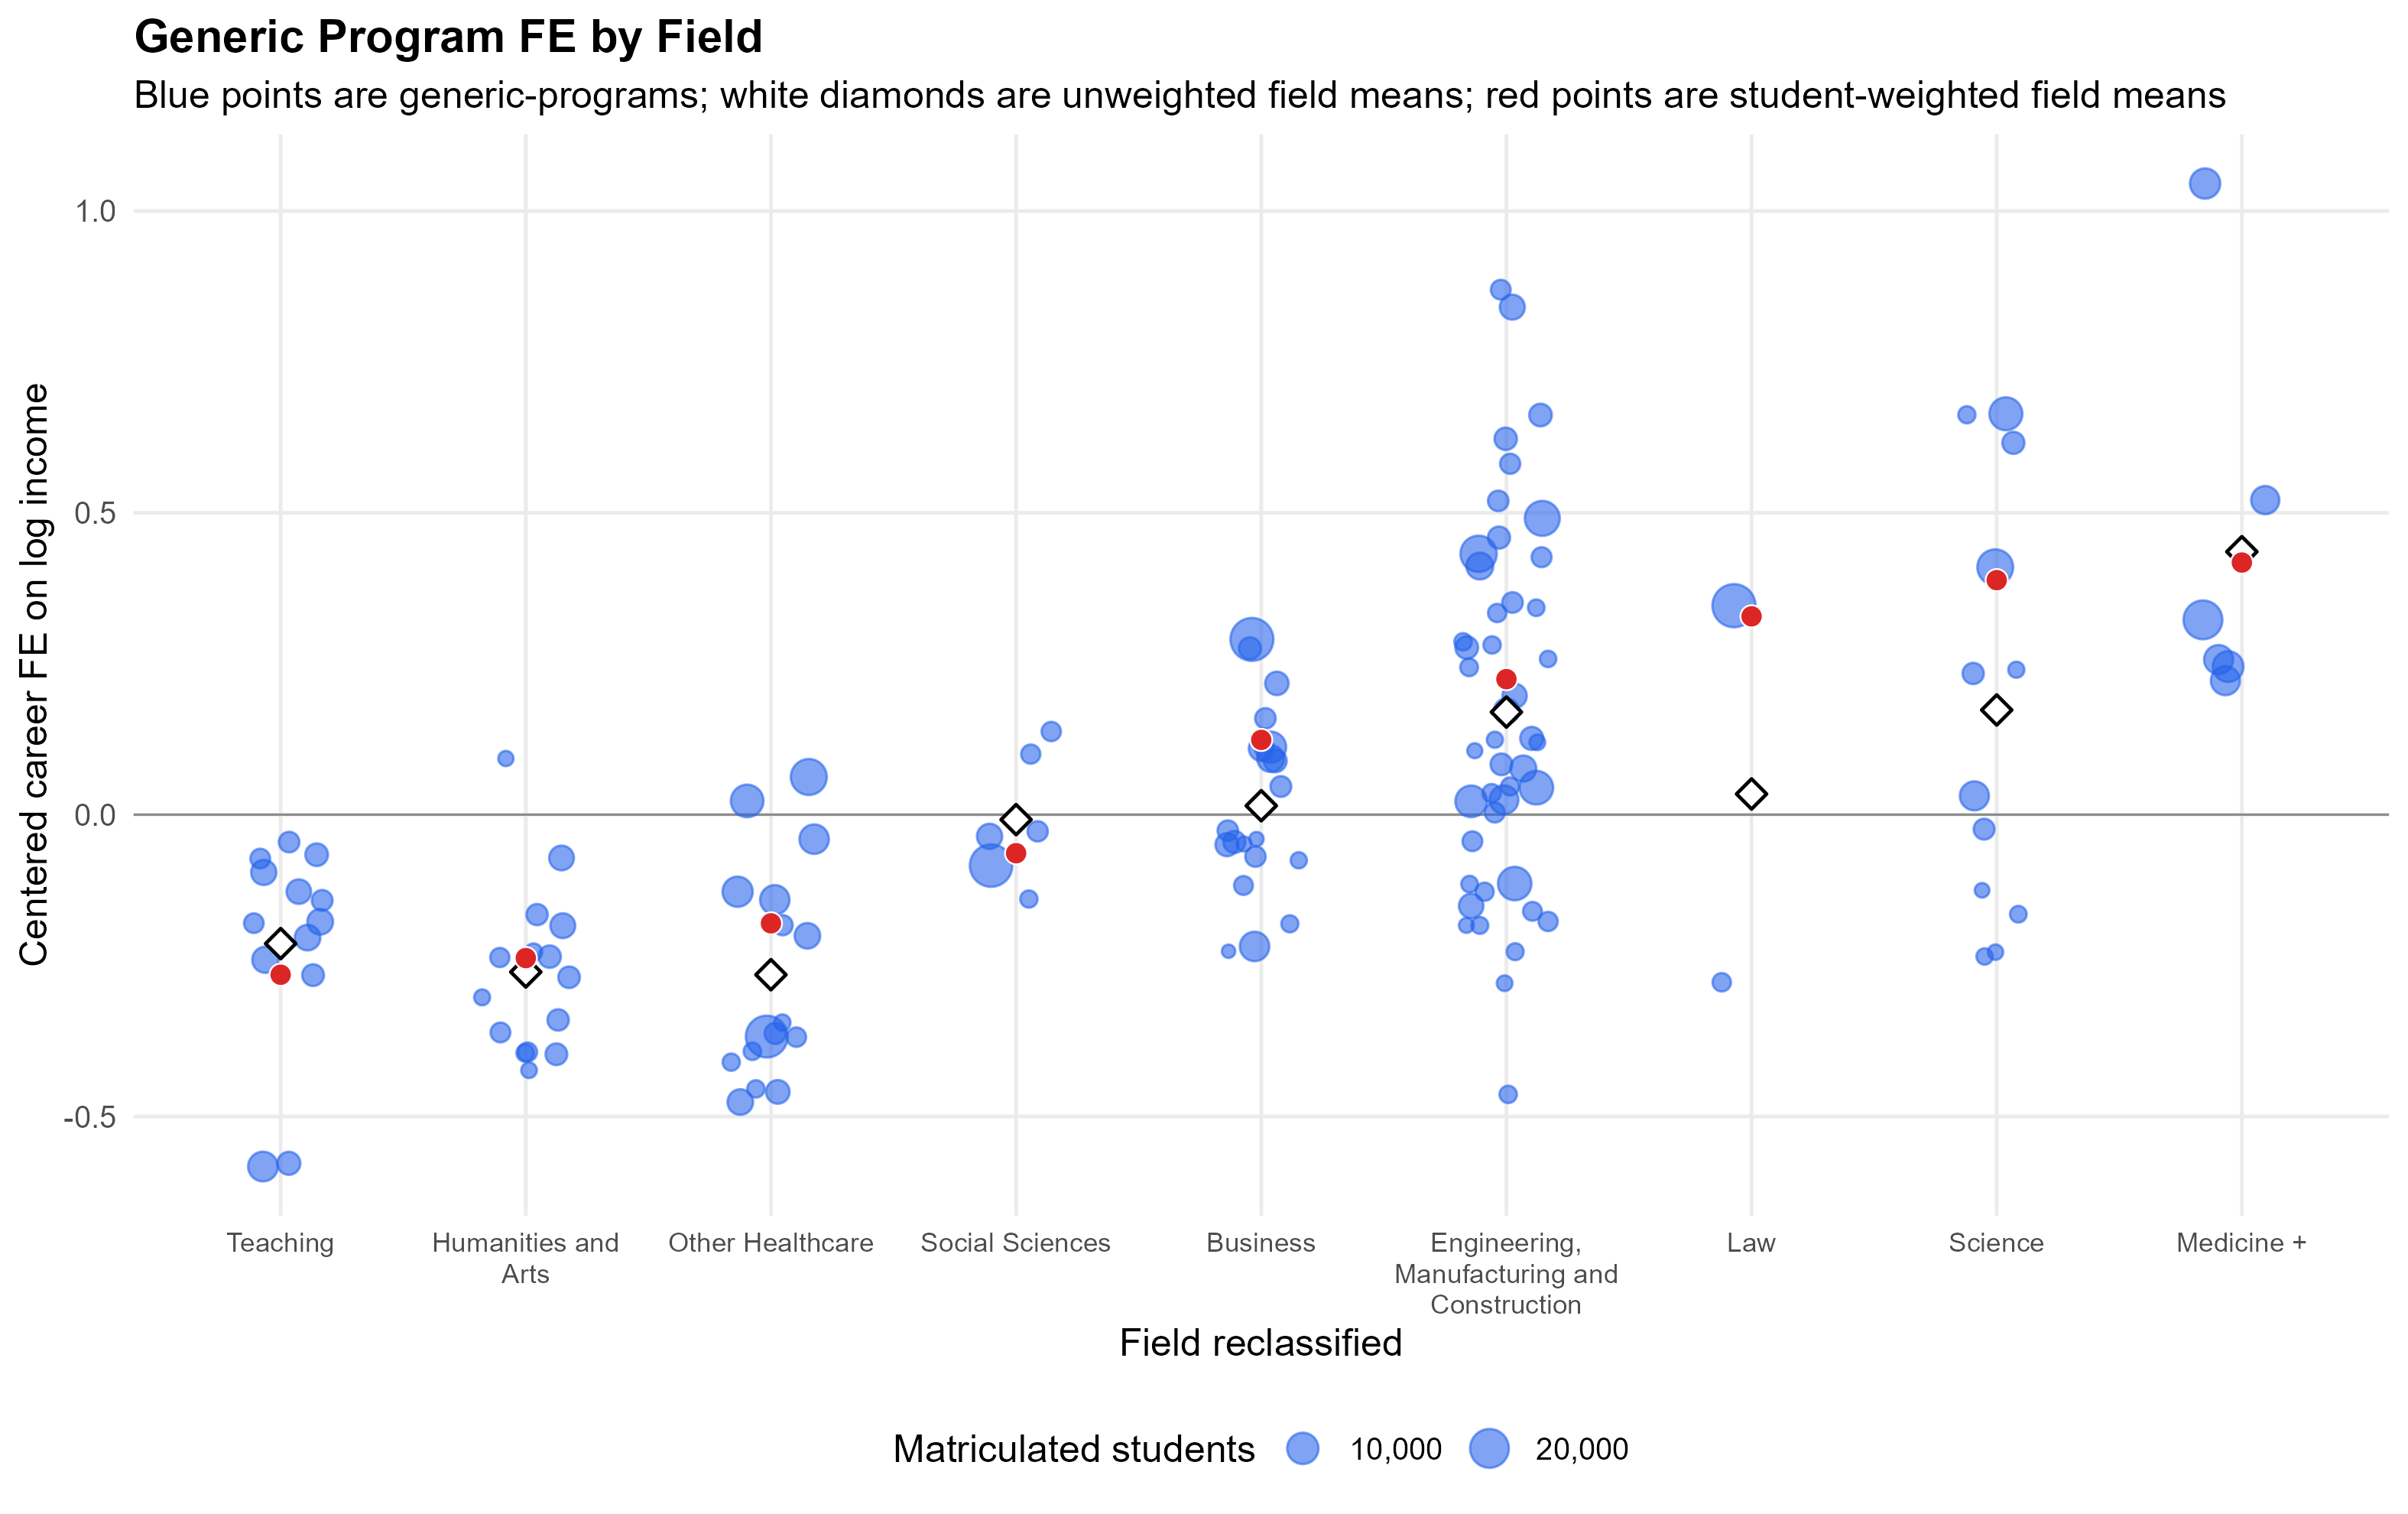
\includegraphics[width=\textwidth]{../../output/figures/mifuturo_matricula_income/area_carrera_generica_program_fe_by_field.png}
\caption{MiFuturo Generic-Program Income Premia by Field}
\label{fig:mifuturo-field-income-premia}
\end{figure}

I link the school panel to higher-education enrollment records for the first observed enrollment.
I use three higher-education choice outcomes.
The first is an indicator for enrollment in a high-premium field.
This indicator equals one for students whose first observed higher-education enrollment is in Science, Law, Engineering/Manufacturing/Construction, or Medicine+\footnote{Medicine+ includes premium health-related careers such as medicine, pharmacy, nursing, midwifery, medical technology, and dentistry.
Other health and technical-health programs are not included in this high-premium-field category.}, which correspond to the right-hand side of Figure~\ref{fig:mifuturo-field-income-premia}.


The second is an indicator for enrollment in a high-premium institution.
This indicator equals one when the student's first observed matriculated institution has a particularly high institution fixed effect in the MiFuturo log-income model.\footnote{Specifically, I use a threshold of 0.1 log points relative to the average program, which roughly translates to an average institution premium of 10\%.}
Students without an observed higher-education enrollment are coded as zero for the high-premium-field and high-premium-institution indicators.

The third is log projected program income.
For matriculated students, projected program income comes from MiFuturo-based predictions using a hierarchy that first uses institution-by-generic-program fixed effects when available, then generic-program fixed effects, then institution fixed effects, and finally the global MiFuturo mean.
For students with no observed higher-education enrollment, projected program income is set to the current minimum-wage proxy of 553,553 Chilean pesos before taking logs.\footnote{This is consistent with the fact that the amounts reported in MiFuturo are in 2025 Chilean pesos.}


%For matriculated students, missing or unsupported high-premium-field classifications are left missing rather than coded as non-high-premium.
%The math and verbal score outcomes require observed national admission-test scores.
%The unconditional postsecondary outcomes instead retain students without higher-education enrollment when non-enrollment is part of the outcome definition.
%In the 2017--2020 complete-control value-added panel, 571,110 students have a math or verbal admission-test outcome.

\clearpage 
\section{Empirical Framework}

This section describes the empirical object and the research design.
The goal is not to estimate a separate causal effect for every school and every possible margin of substitution.
Instead, I ask whether an outcome-specific observational value-added measure is informative about causal effects generated by lottery-induced changes in school attendance.
The design therefore collapses school effects into scalar measures and estimates a forecast coefficient for each outcome.

\subsection{School Effects and Observational Value Added}

I use a constant-effects value-added model as a guide:
\begin{equation}
  Y_i^m(j) = \mu^m + V_j^m + \epsilon_i^m,
  \label{eq:potential-va}
\end{equation}
Here, $Y_i^m(j)$ is student $i$'s potential outcome for outcome $m$ if assigned to high school $j$.
The index $m$ denotes the outcome, and $j$ denotes the high school.
The term $\mu^m$ is the average level of outcome $m$ under the student-weighted average school.
The term $V_j^m$ is the contribution of school $j$ to outcome $m$ relative to that average.
The term $\epsilon_i^m$ captures student-level determinants of outcome $m$ that do not vary with the assigned school in this constant-effects representation.
I normalize school effects so that their student-weighted mean is zero, $\sum_j \omega_j V_j^m = 0$, where $\omega_j$ is the share of students linked to school $j$ in the value-added sample.
This centering means that the weighted average of $V_j^m$ across schools is exactly zero.
A positive $V_j^m$ therefore denotes a school above the student-weighted average for outcome $m$, while a negative value denotes a school below that average.
The main outcomes are math and verbal achievement, indicators for enrollment in a high-premium field and a high-premium institution, and log projected program income. 

The first step constructs observational value added in the broad complete-control panel.
For each outcome $m$, I estimate
\begin{equation}
  Y_i^m = \alpha^m + \lambda_{s(i)}^m + X_i'\Gamma^m + u_i^m,
  \label{eq:observational-va}
\end{equation}
where $s(i)$ is the student's main high-school RBD and $X_i$ contains pre-treatment controls.
These include cohort, gender, age, a third-degree polynomial in each of grade-4 SIMCE math and language, family-background measures from SIMCE parent surveys\footnote{In particular: family income decile, years of education and indigenous status of each parent, and indicators for whether the student attended any institution before primary education.}, and middle-school controls from grades 5 to 8 (middle school indicator and school-normalized attendance and performance).
%Score outcomes are estimated among students with observed admission-test scores, while the other postsecondary outcomes use the complete-control panel after applying the outcome-specific missing-data rules described above.
I define the observational value-added measure $\widehat{V}_j^m$ as the centered empirical analogue of $V_j^m$: the estimated school fixed effect $\widehat{\lambda}_j^m$ from equation~\eqref{eq:observational-va}, centered using the same student-weighting convention.

Importantly, these fixed effects by themselves answer an observational question: conditional on $X_i$, which schools have higher average outcomes?
If school assignment in the broad panel were truly random, then the centered fixed effect $\widehat{\lambda}_j^m$ would identify $V_j^m$ up to sampling error.
In practice, students sort across schools, so the fixed effects may combine true school effects with any remaining selection not absorbed by controls.
The second step therefore asks whether the part of $\widehat{V}_j^m$ shifted by the SAE lotteries corresponds to causal effects in the same outcome.


\subsection{Assignment Risk and Expected Value Added}

SAE applicants submit rank-ordered lists of schools.
Let $Z_i$ denote the first-round school offer and $D_i$ denote the school attended, measured by the post-grade-8 most-time RBD.
A student has a preference and priority type $\theta_i$, and the assignment mechanism implies an assignment-probability vector $p_i=(p_{i1},...,p_{iJ})$, where $p_{ij}=Pr(Z_i=j)$.
Under equal treatment of equals, students with the same type have the same assignment probabilities \parencite{abdulkadiroglu_research_2017}.
For pre-treatment characteristics and potential outcomes fixed under re-randomization, we have
\begin{equation}
  (Y_i^m(1),...,Y_i^m(J), X_i) \ind Z_i \mid p_i.
  \label{eq:offer-independence}
\end{equation}

The raw vector $p_i$ is high-dimensional, because students can rank many different combinations of schools.
For an outcome-specific scalar value-added measure, I summarize assignment risk by the expected value added in the student's portfolio:
\begin{equation}
  E_i^m = \sum_j p_{ij}\widehat{V}_j^m.
  \label{eq:expected-va}
\end{equation}
This is the average value added the student would receive over repeated randomizations of the assignment mechanism, holding the submitted application and priorities fixed.
In the main IV specification, this scalar expected value replaces a large set of school-specific probability controls.

For each outcome $m$, define the value added of the attended school and offered school as
\begin{equation}
  A_i^m = \widehat{V}_{D_i}^m,
  \qquad
  O_i^m = \widehat{V}_{Z_i}^m.
  \label{eq:attended-offered-va}
\end{equation}
The instrument is $O_i^m$, the value added of the school generated by the lottery offer.
The endogenous variable is $A_i^m$, the value added of the school actually attended.
The notation is mnemonic: $O_i^m$ is the value added of the \textbf{O}ffered school, and $A_i^m$ is the value added of the \textbf{A}ttended school.
Because assignment offers vary randomly conditional on the assignment probabilities, variation in $O_i^m$ around $E_i^m$ provides quasi-experimental variation in the quality of the school offer.


\subsection{Scalar IV Specification}

The first empirical question is whether observational value added predicts causal effects on the same outcome.
Specifically, when the assignment mechanism moves a student toward a school with higher $\widehat{V}_j^m$, does outcome $m$ rise, and by how much relative to the observational difference encoded in $\widehat{V}_j^m$?
The main IV system is given by the following pair of equations:
\noindent
  \begin{equation}
    \begin{aligned}
      Y_i^m ={}& \alpha^m + \theta^m A_i^m + \rho^m E_i^m +  W_i'\delta^m + \eta_i^m,
    \end{aligned}
    \label{eq:pass-through}
  \end{equation}

  \begin{equation}
    \begin{aligned}
      A_i^m ={}& a^m + \kappa^m O_i^m + \rho_A^m E_i^m +  W_i'\delta_A^m + \nu_i^m.
    \end{aligned}
    \label{eq:first-stage}
  \end{equation}

Here, $Y_i^m$ is student $i$'s realized value of outcome $m$. The value added of the attended school, $A_i^m$, is instrumented with the value added of the school offered through the assignment mechanism, $O_i^m$.
$E_i^m$ is the expected value added implied by the student's assignment-probability vector.
Finally, $W_i$ is a parsimonious lottery-sample control vector containing cohort, gender, age, and grade-4 SIMCE math and language.
This differs from the richer control vector used to construct $\widehat{V}_j^m$ in equation~\eqref{eq:observational-va}, which also includes family-background and middle-school controls.
%The rich controls enter through the construction of the school value-added measures, while equation~\eqref{eq:pass-through} asks whether those pre-constructed measures pass through in the SAE lottery sample after conditioning on assignment risk and core baseline covariates.
All reported specifications use heteroskedasticity-robust standard errors.

The coefficient $\theta^m$ is the key object.
It measures how much of the observational value-added difference induced by the lottery offer passes through into causal effects on the same outcome.
If $\theta^m=1$, then a one-unit increase in observational value added causes a one-unit increase in the outcome.
If $\theta^m=0$, the observational measure has no causal predictive content along the lottery-induced margin.
Values between zero and one imply that observational value added is directionally informative, but overstates the causal effect of attending higher-value-added schools.

The scalar design is useful because a fully flexible school-specific IV design would be high-dimensional and would mix many margins of substitution across fallback schools \parencite{angrist_methods_2023, kirkeboen_field_2016}.
It instead asks whether movement toward schools with higher measured value added causes better outcomes, after controlling for the expected value added implied by each student's assignment risk.

A second empirical question is whether the forecast differs by students' baseline achievement.
To answer that question, I also estimate equation~\eqref{eq:pass-through} separately by quintiles of baseline grade-4 math achievement or gender.
Evidently since gender and grade-4 SIMCE are fixed before high-school assignment, these splits describe heterogeneity without conditioning on a post-treatment outcome.

\subsection{Empirical Bayes}

The school fixed effects in equation~\eqref{eq:observational-va} are estimated with different precision.
In particular, effects for schools with smaller regression samples or noisier outcomes contain more sampling error.
I therefore use an Empirical-Bayes (EB) version of the observational school-value index, which shrinks noisier estimates more strongly toward the across-school mean \parencite{walters_chapter_2024}.
For each outcome $m$, let $se_j^m$ denote the regression-derived standard error of the student-weighted centered fixed effect $\widehat{V}_j^m$.
This is the uncertainty of the same centered effect used in the scalar design, rather than the standard error of an arbitrary reference-normalized school dummy.

I estimate the latent across-school variance by subtracting average sampling variance from the student-weighted variance of the estimated effects:
\begin{equation}
  \widehat{\tau}_m^2 =
  \max\left\{
    \operatorname{Var}_{\omega}\left(\widehat{V}_j^m\right)
    - \sum_j \omega_j (se_j^m)^2,\,
    0
  \right\},
  \label{eq:eb-latent-variance}
\end{equation}
where $\omega_j$ is proportional to the number of students in school $j$'s stage-1 regression sample.
The implied school-specific reliability is
\begin{equation}
  \lambda_j^m =
  \frac{\widehat{\tau}_m^2}
  {\widehat{\tau}_m^2 + (se_j^m)^2},
  \label{eq:eb-reliability}
\end{equation}
and the EB school value is
\begin{equation}
  \widehat{V}_{j}^{m,EB}
  =
  \overline{\widehat{V}}_{\omega}^m
  +
  \lambda_j^m
  \left(
    \widehat{V}_j^m-\overline{\widehat{V}}_{\omega}^m
  \right).
  \label{eq:eb-va}
\end{equation}
Note that as $(se_j^m) \to 0$ (more precision on the estimate), $\lambda^m_j \to 1$ and the posterior approaches the original $\hat{V}_j^m$.
Otherwise, the posterior lies between the estimate $\hat{V}_j^m$ and the mean of such estimates $\overline{\hat{V}_j^m}$.

I recenter these posterior means using the same student weights, so their student-weighted mean remains zero.

I then replace $\widehat{V}_j^m$ with $\widehat{V}_{j}^{m,EB}$ everywhere in the scalar IV construction:
\begin{equation}
  A_i^{m,EB} = \widehat{V}_{D_i}^{m,EB},
  \qquad
  O_i^{m,EB} = \widehat{V}_{Z_i}^{m,EB},
  \qquad
  E_i^{m,EB} = \sum_j p_{ij}\widehat{V}_{j}^{m,EB}.
  \label{eq:eb-iv-objects}
\end{equation}
The EB specification instruments $A_i^{m,EB}$ with $O_i^{m,EB}$ and controls for $E_i^{m,EB}$ in the same way as equation~\eqref{eq:pass-through}.
%Thus, EB improves the signal-to-noise ratio of the stage-1 observational index before it is used in the lottery design; it does not estimate a separate causal effect for each school or form a hybrid causal-EB estimator.
%Because shrinkage compresses the scale of the school-value index, the resulting forecast coefficients should be interpreted together with the distribution of the EB-shrunken index.


\subsection{Ordered Value-Added Horse Race}

The final empirical question asks which school-value dimensions best predict gains in projected program income, and in particular how much of that signal is captured by math achievement value added.
Projected income is a composite earnings proxy: it can rise because students enroll in higher education at higher rates, because they enter high-premium institutions, or because they enter high-premium fields.
Moreover, all such effects might be a direct consequence of higher achievement.

Let $\widehat{V}_j^{M}$ denote math EB value added, $\widehat{V}_j^{I}$ high-premium-institution EB value added, and $\widehat{V}_j^{F}$ high-premium-field EB value added.
To make the joint exercise easier to interpret, I use an ordered residualization of the three school-level measures.
Math value added enters first.
High-premium-institution value added is residualized on math value added.
High-premium-field value added is then residualized on both math value added and the institution component.
The ordering is therefore math, high-premium institution, and high-premium field.
It is meant only as an interpretation device: the exercise asks whether each later dimension adds predictive content for projected income beyond the earlier dimensions in this order.

For each student, I merge these ordered school-value measures to the attended high school, the first-round offered school, and the DA assignment-probability portfolio:
\begin{equation}
  \begin{aligned}
  A_i^k &= \widetilde{V}_{D_i}^{k},\\
  O_i^k &= \widetilde{V}_{Z_i}^{k},\\
  E_i^k &= \sum_j p_{ij}\widetilde{V}_{j}^{k},
  \qquad k \in \{M,I \perp M,F \perp M,I\}.
  \end{aligned}
  \label{eq:ordered-va-objects}
\end{equation}
Here $D_i$ is the attended high school, $Z_i$ is the first-round offered school, and $p_{ij}$ is the DA assignment probability for school $j$.

I then estimate a joint IV model for log projected program income in which the three ordered value-added measures enter together.
The attended values are endogenous treatments, the offered values are instruments, and the expected values are included as assignment-risk controls:
\begin{equation}
  Y_i^{PI} =
  \alpha
  + \big( 
    \theta_M A_i^{M}
  + \rho_M E_i^{M} 
    \big) 
  + \big( 
   \theta_I A_i^{I \perp M}
  + \rho_I E_i^{I \perp M}
    \big) 
  + \big(   
   \theta_F A_i^{F \perp M,I}
  + \rho_F E_i^{F \perp M,I}
      \big) 
  + W_i'\delta
  + \eta_i.
  \label{eq:ordered-va-iv}
\end{equation}
This specification is an ordered horse race among school value-added dimensions.
It asks whether the lottery-based signal for projected program income is carried mainly by achievement value added or whether higher-education choice dimensions also play an important role.
The coefficients are therefore not structural returns to test scores, institutions, or fields themselves.
Instead, they show which school value-added dimensions have predictive content for projected income after accounting for the earlier dimensions in the chosen order.


\clearpage 
\section{Results}

I organize the results in five blocks.
First, I describe the scale of the underlying outcomes and the distribution of the five primary observational school value-added measures.
Second, I report the main forecast coefficient estimates for each outcome.
Third, I examine heterogeneity in forecast by baseline grade-4 math achievement.
Fourth, I examine whether pass-through differs by student gender.
Finally, I use an ordered value-added horse race to compare achievement, high-premium-institution, and high-premium-field dimensions of school value added when predicting projected program income.

\subsection{Distribution of Value-Added Estimates}

Table~\ref{tab:school-va-distribution} reports the mean and standard deviation of each underlying student outcome alongside the student-weighted distribution of the corresponding school value-added measure.
The former capture variation across students; the latter capture estimated differences in school contributions.

\begin{table}[!htbp]
\centering
\begin{threeparttable}
\caption{Distribution of primary EB-shrunken school value added}
\label{tab:school-va-distribution}
\footnotesize
\setlength{\tabcolsep}{2pt}
\begin{tabular}{lcc|cccccc}
\toprule
 & \multicolumn{2}{c|}{Outcome distribution} & \multicolumn{6}{c}{Value-added distribution} \\
\cmidrule(lr){2-3} \cmidrule(lr){4-9}
Outcome & \shortstack{Sample\\Mean} & \shortstack{Sample\\SD} & VA SD & P10 & P25 & P50 & P75 & P90 \\
\midrule
Math & 0.043 & 1.002 & 0.222 & -0.195 & -0.141 & -0.062 & 0.057 & 0.297 \\
Verbal & 0.049 & 0.989 & 0.150 & -0.172 & -0.111 & -0.021 & 0.083 & 0.202 \\
High-premium institution & 0.142 & 0.349 & 0.106 & -0.090 & -0.066 & -0.029 & 0.023 & 0.144 \\
High-premium field & 0.347 & 0.476 & 0.053 & -0.060 & -0.035 & -0.004 & 0.030 & 0.063 \\
Log proj. income & 13.893 & 0.522 & 0.072 & -0.093 & -0.049 & -0.002 & 0.044 & 0.090 \\
\bottomrule
\end{tabular}
\begin{tablenotes}[flushleft]
\footnotesize
\item[] \parbox{0.84\textwidth}{Notes: The table reports student-weighted distributions of EB-shrunken, student-centered school value added. Schools are weighted by the number of students in the corresponding Stata value-added regression. Sample moments refer to the outcome-specific value-added regression sample. Math and verbal are measured in admission-test standard deviations; the two high-return outcomes are binary; projected program income is measured in logs.}
\end{tablenotes}
\end{threeparttable}
\end{table}


The achievement outcomes are standardized measures, so their sample means are close to zero and their standard deviations are close to one.
The probability of entering a high-premium institution is 0.142, and the probability of entering a high-premium field is 0.347.
Mean log projected program income is 13.893, with a student-level standard deviation of 0.522.

The school value-added measures also display substantial dispersion.
The standard deviation of math value added is 0.222, and the gap between the 90th and 10th percentiles is 0.492 standard deviations.
For verbal, the corresponding standard deviation is 0.150 and the 90--10 gap is 0.374 standard deviations.
Among the higher-education outcomes, the standard deviation of high-premium-institution value added is 0.106, and the corresponding standard deviation for high-premium-field value added is 0.053.
Projected-income value added has a standard deviation of 0.072 log points and a 90--10 gap of 0.184 log points.
These distributions show that the observational measures contain economically meaningful variation and provide the scale needed to interpret the pass-through estimates below.

\subsection{IV Estimates}


Table~\ref{tab:scalar_school_value_iv_main_five_expected_va_eb} reports the five primary EB IV estimates.
Each column uses the same outcome to construct the observational school value-added measure, the first-round offered-school value-added instrument, and the realized attended-school value-added treatment.
The coefficients can therefore be read as pass-through estimates: how much a lottery-induced increase in a school's observational value added translates into a causal gain in the corresponding student outcome.

The value-added metrics contain important signal: I reject $\theta = 0$ in all dimensions of value added.

The achievement estimates are close to one: a one-unit increase in the EB math value-added index raises math achievement by 0.884 standard deviations, while the analogous estimate for verbal is 0.885.
Moreover, the achievement estimates are close to comparable lottery-based estimates in \textcite{angrist_leveraging_2017}, despite the absence of immediately lagged outcomes.
This result supports the richness of the pre-treatment controls used in this design, since they deliver results similar to settings where immediate lagged measures are available.
This reasoning should also give confidence in the non-achievement estimates, since they use the same rich control vector.

The estimated pass-through is 0.497 for high-premium-institution enrollment, 0.803 for high-premium-field enrollment, and 0.311 for projected program income.
Yet the relatively low forecast coefficients for high-premium-institution enrollment and program income suggest an important degree of noise in those measures of value added.

Taken together, the estimates suggest that the observational school value-added measures are informative about both test-score production and later higher-education choices.
They also provide lottery-based evidence that high schools causally affect all five primary outcomes studied here.
Lottery-induced movement toward schools with higher observational value added raises math achievement, verbal achievement, entry into high-premium institutions and high-premium fields, and projected program income, although at different rates depending on the outcome.
The results therefore show that the school assignment margin shifts later higher-education choices, not only test scores.

\begin{table}[!htbp]
\centering
\caption{Main scalar school-value IV estimates using EB-shrunken value added}
\label{tab:scalar_school_value_iv_main_five_expected_va_eb}
\resizebox{\textwidth}{!}{%
\begin{tabular}{lccccc}
\toprule
 & \multicolumn{2}{c}{Exams} & \multicolumn{3}{c}{Higher ed. choices} \\
\cmidrule(lr){2-3} \cmidrule(lr){4-6}
 & Math & Verbal & High-premium inst. & High-premium field & Program income \\
\midrule
$\theta^{EB}$ & 0.884*** & 0.885*** & 0.497*** & 0.803*** & 0.311*** \\
 & (0.073) & (0.087) & (0.111) & (0.100) & (0.103) \\
N & 93,438 & 95,107 & 95,651 & 90,338 & 95,651 \\
\bottomrule
\end{tabular}
}
\par\medskip
\footnotesize
\begin{minipage}{\textwidth}
Notes: Each column reports a scalar IV estimate of the pass-through from attended-school EB value added to the corresponding student outcome. Attended-school EB value added is instrumented with first-round offered-school EB value added. All specifications control for the DA-probability expected value of the same EB measure, cohort, grade-4 SIMCE math and language, gender, and age. Heteroskedasticity-robust standard errors are reported in parentheses. $^{*}p<0.10$, $^{**}p<0.05$, $^{***}p<0.01$.
\end{minipage}
\end{table}



\subsection{Heterogeneity by Baseline Achievement}

Figure~\ref{fig:simce4-math-quintile-primary-five-eb} repeats the five primary EB estimates separately by quintiles of baseline grade-4 math achievement.
This comparison is useful because it keeps the heterogeneity split pre-treatment and available for the full exam-taker analysis sample.
Table~\ref{tab:simce4-math-quintile-primary-five-eb-contrasts-q3} formally tests each quintile coefficient against the middle quintile, reporting $\widehat{\theta}^{EB}_{Q_q}-\widehat{\theta}^{EB}_{Q_3}$ for $q\in\{1,2,4,5\}$.

The clearest heterogeneity appears in math.
The bottom-quintile estimate is 0.083, compared with 0.929 in the middle quintile, a difference of $-0.846$ ($p<0.01$).
The top-quintile estimate is 1.285, or 0.356 above the middle quintile, although this difference is significant only at the 10 percent level ($p=0.093$).
The math estimates for the second and fourth quintiles are not statistically different from the middle-quintile estimate.
These results suggest a limit to the constant-effects model of schools, but also efficiency and equity considerations on policies based on value-added reporting.
Low baseline achievement students might severely underestimate the gains from switching schools, rendering those moves as less efficient or even detrimental if we consider switching costs.

None of the four contrasts with the middle quintile is statistically significant for verbal, high-premium-institution enrollment, high-premium-field enrollment, or log projected program income.
Thus, the formal tests support meaningful heterogeneity in math, but an almost flat gradient across the higher-education outcomes by baseline achievement.

\begin{figure}[!htbp]
\centering
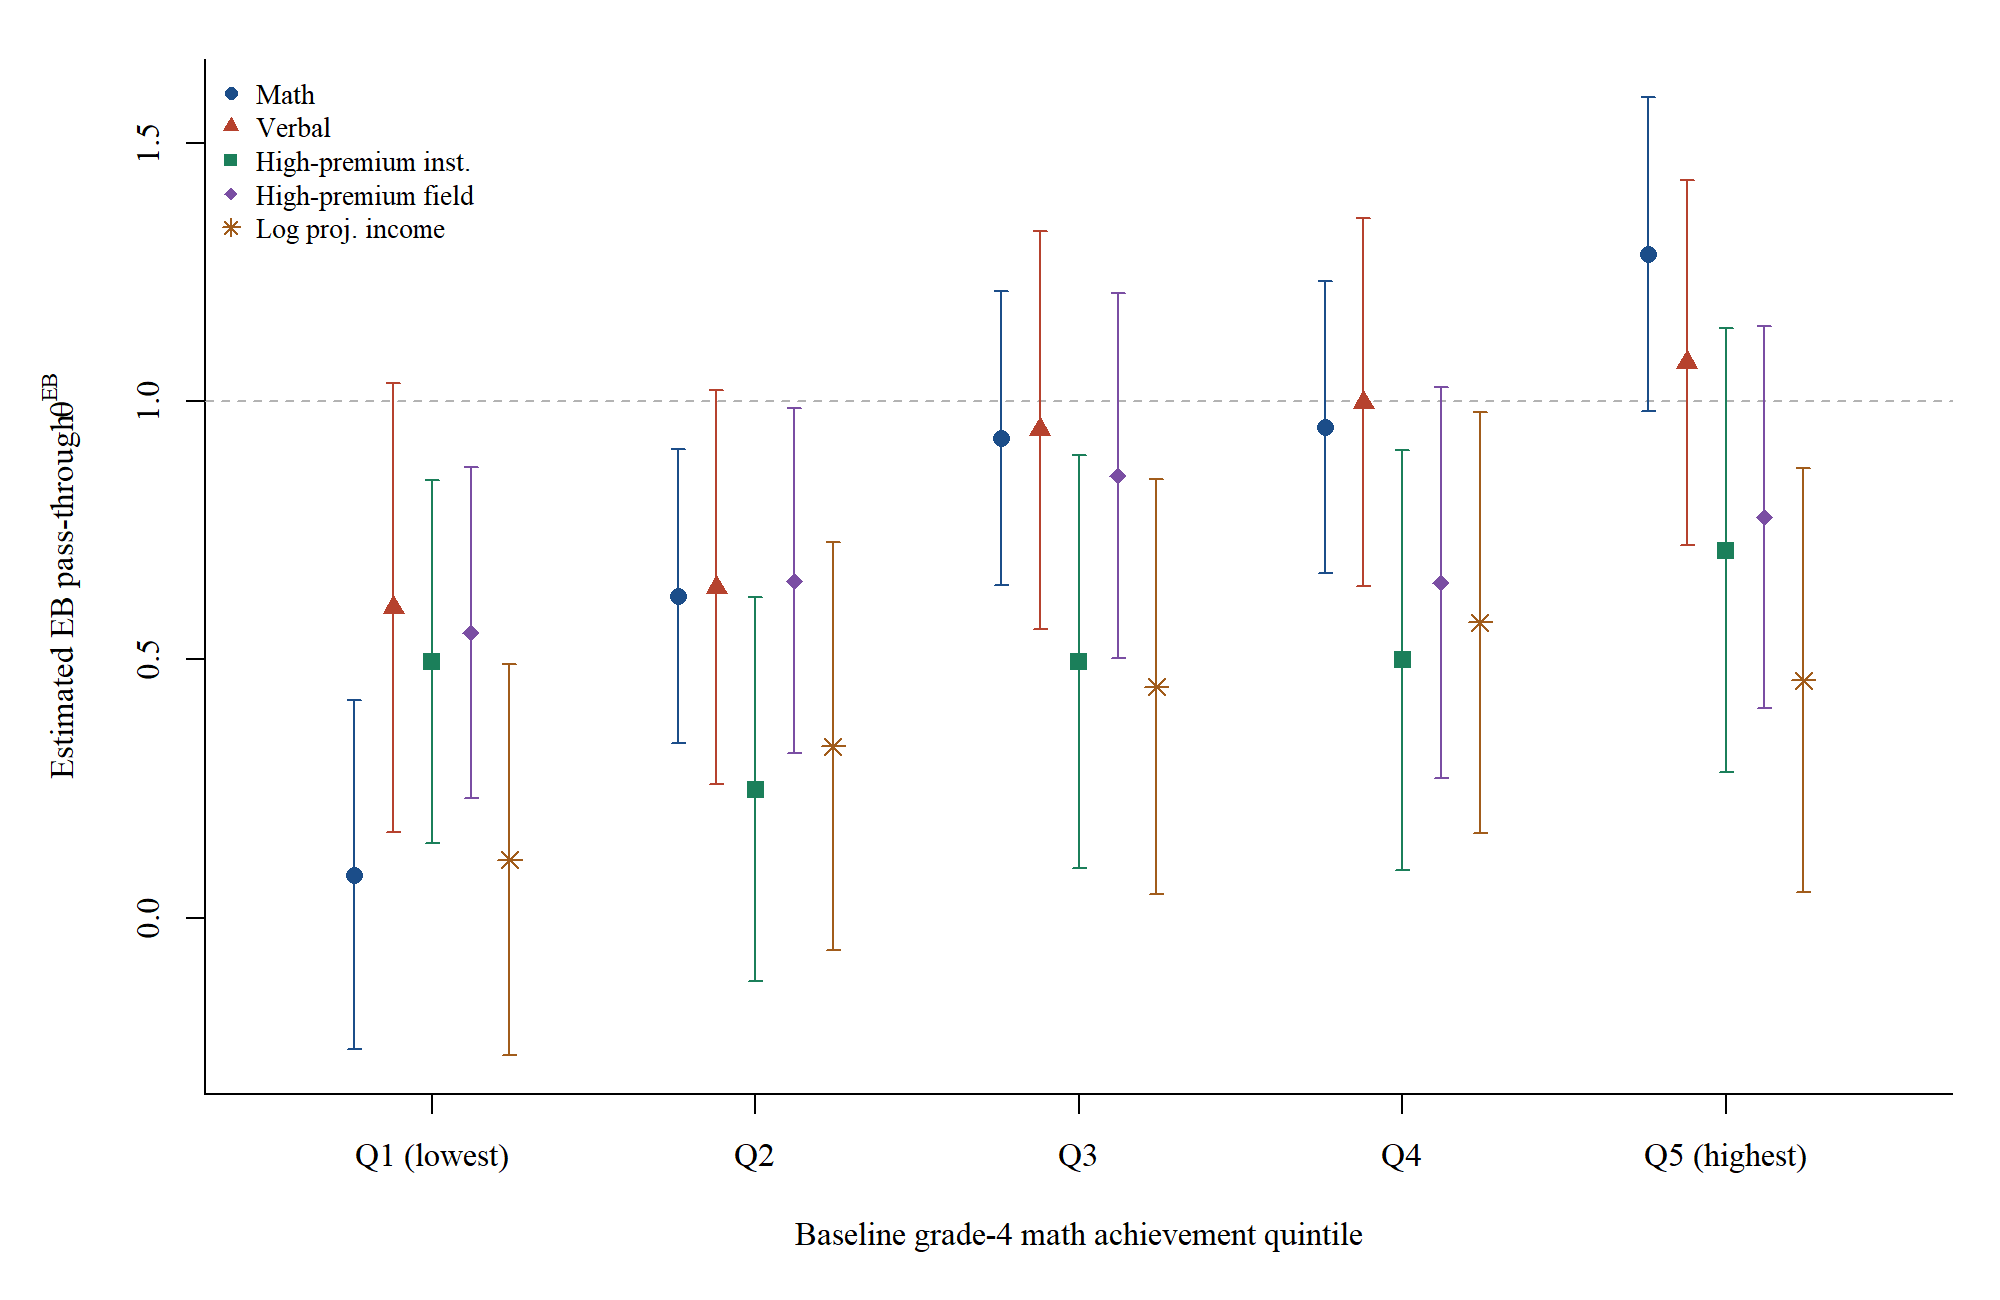
\includegraphics[width=.9\textwidth]{../../output/figures/results_section/simce4_math_quintile_primary_five_eb.png}
\caption{EB scalar school-value IV estimates by baseline grade-4 math achievement quintile}
\label{fig:simce4-math-quintile-primary-five-eb}
\end{figure}
\begin{table}[!htbp]
\centering
\caption{Differences in EB pass-through relative to the middle quintile}
\label{tab:simce4-math-quintile-primary-five-eb-contrasts-q3}
\small
\resizebox{\textwidth}{!}{%
\begin{tabular}{lccccc}
\toprule
 & \multicolumn{2}{c}{Exams} & \multicolumn{3}{c}{Higher ed. choices} \\
\cmidrule(lr){2-3} \cmidrule(lr){4-6}
Comparison & Math & Verbal & High-premium inst. & High-premium field & Log proj. income \\
\midrule
$Q1-Q3$ & -0.846*** & -0.345 & 0.001 & -0.304 & -0.335 \\
 & (0.225) & (0.296) & (0.272) & (0.243) & (0.282) \\
$Q2-Q3$ & -0.306 & -0.305 & -0.247 & -0.203 & -0.115 \\
 & (0.205) & (0.277) & (0.278) & (0.248) & (0.287) \\
$Q4-Q3$ & 0.022 & 0.053 & 0.003 & -0.207 & 0.125 \\
 & (0.205) & (0.268) & (0.291) & (0.264) & (0.292) \\
$Q5-Q3$ & 0.356* & 0.130 & 0.216 & -0.080 & 0.013 \\
 & (0.212) & (0.267) & (0.300) & (0.261) & (0.293) \\
\bottomrule
\end{tabular}
}
\par\medskip
\footnotesize
\begin{minipage}{\textwidth}
Notes: Each entry reports $\widehat{\theta}^{EB}_{Q_q} - \widehat{\theta}^{EB}_{Q3}$ for the indicated baseline grade-4 math achievement quintile. Heteroskedasticity-robust standard errors are reported in parentheses. Because quintile samples are disjoint, the contrast variance is the sum of the two coefficient variances. $^{*}p<0.10$, $^{**}p<0.05$, $^{***}p<0.01$.
\end{minipage}
\end{table}

\FloatBarrier

\subsection{Heterogeneity by Gender}

I next ask whether the forecast estimates differ by gender.
Gender is measured from the grade-8 enrollment records used to construct the linked student panel, so this split is predetermined relative to high-school assignment and does not rely on SAE or admission-test records.
Figure~\ref{fig:primary-five-eb-by-gender} reports the five EB forecast estimates separately for boys and girls.
Table~\ref{tab:primary-five-eb-gender-contrasts} reports the corresponding difference, girls relative to boys.

The estimates are positive for both groups across all five outcomes.
For achievement, however, the point estimates are larger for girls.
The math pass-through estimate is 0.703 for boys and 1.053 for girls, a difference of 0.349 ($p=0.017$).
The verbal estimate is 0.685 for boys and 1.066 for girls, a difference of 0.382 ($p=0.029$).
Thus, lottery-induced movement toward schools with higher achievement value added appears to translate more strongly into measured achievement gains for girls.

For higher-education choices, the gender differences are noticeably smaller.
The point estimates for high-premium-institution enrollment and high-premium-field enrollment are also larger for girls, but neither difference is statistically significant.
For log projected program income, the point estimate is slightly larger for boys, and the difference is close to zero.
Overall, the gender split suggests meaningful heterogeneity in achievement pass-through, but does not provide evidence that the school effects on higher-education choices differ systematically between boys and girls.

\begin{figure}[!htbp]
\centering
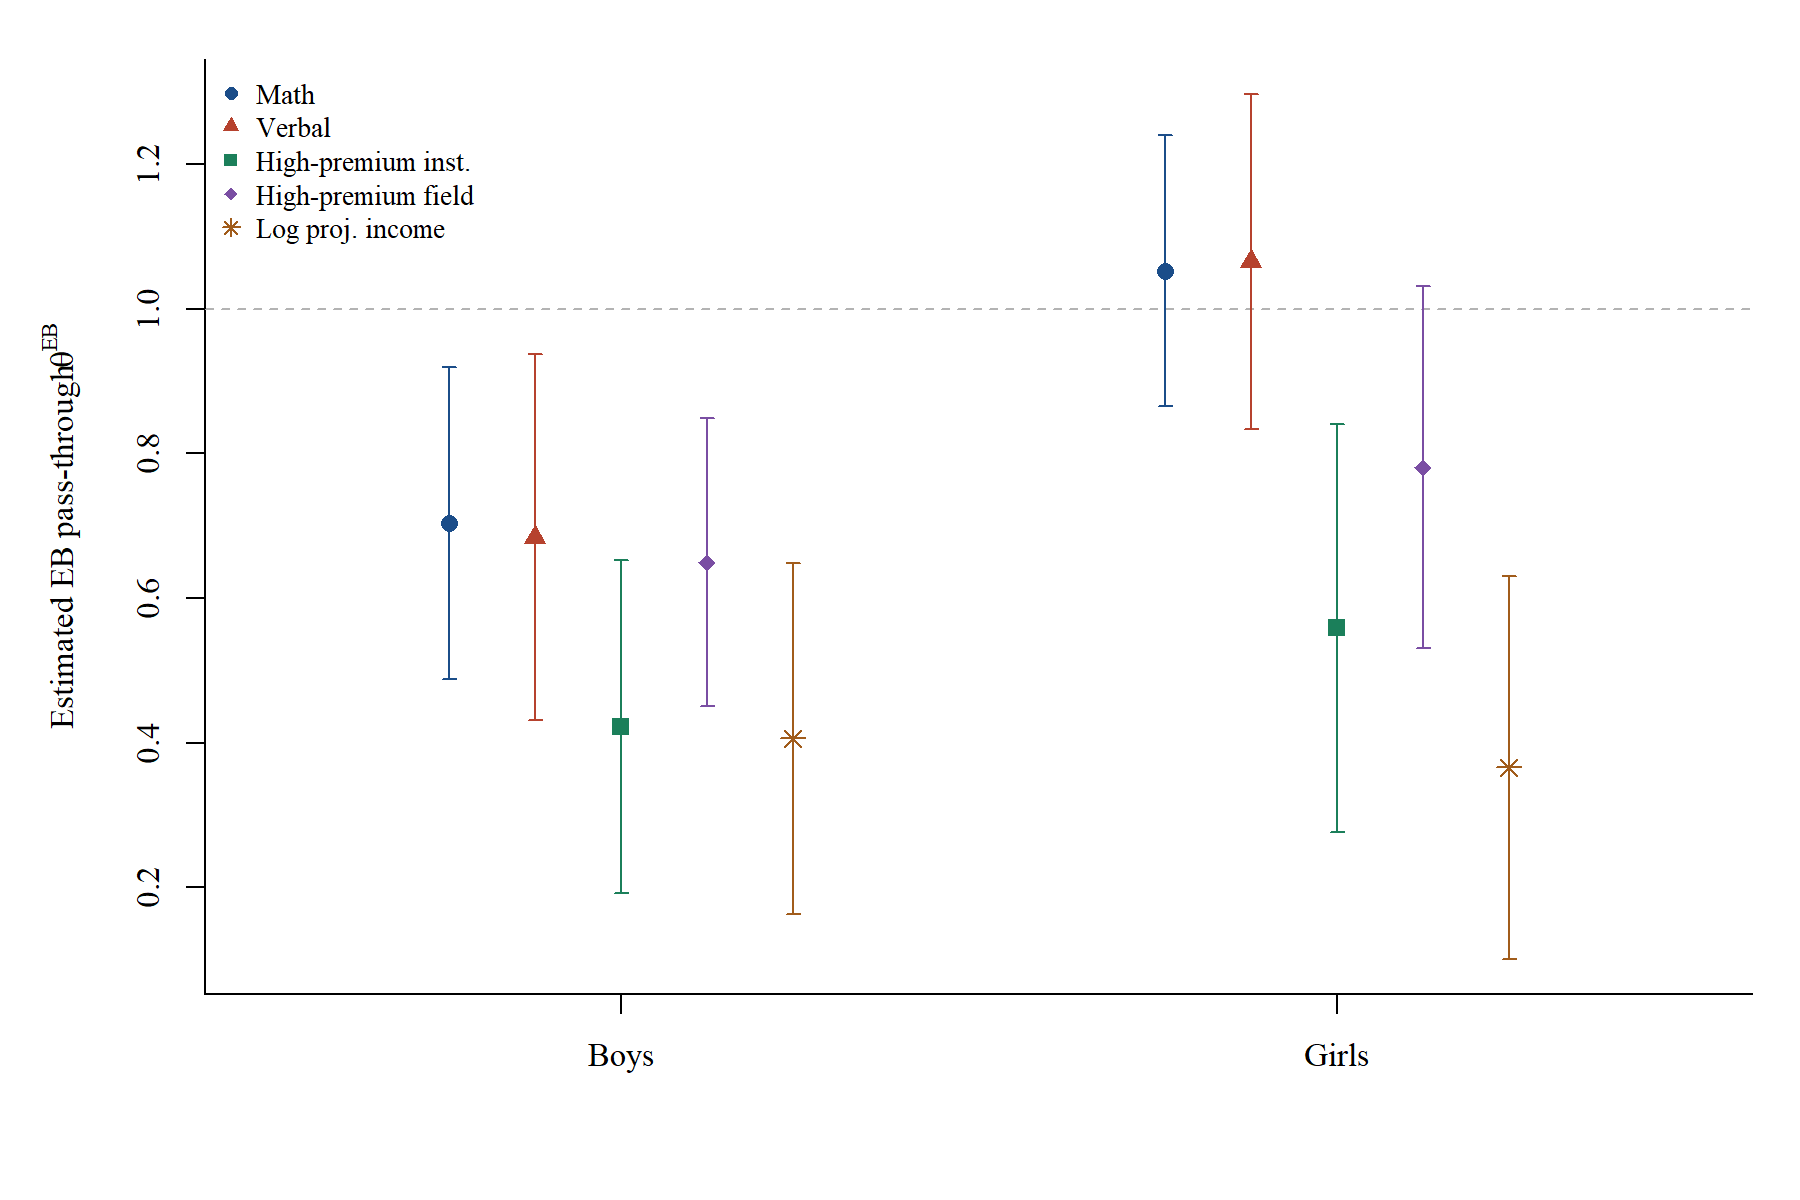
\includegraphics[width=.9\textwidth]{../../output/figures/results_section/primary_five_eb_by_gender.png}
\caption{EB scalar school-value IV estimates by gender}
\label{fig:primary-five-eb-by-gender}
\end{figure}
\begin{table}[!htbp]
\centering
\caption{Gender differences in EB pass-through}
\label{tab:primary-five-eb-gender-contrasts}
\small
\resizebox{\textwidth}{!}{%
\begin{tabular}{lccccc}
\toprule
 & \multicolumn{2}{c}{Exams} & \multicolumn{3}{c}{Higher ed. choices} \\
\cmidrule(lr){2-3} \cmidrule(lr){4-6}
Comparison & Math & Verbal & High-premium inst. & High-premium field & Log proj. income \\
\midrule
Girls $-$ Boys & 0.349** & 0.382** & 0.137 & 0.131 & -0.040 \\
 & (0.146) & (0.175) & (0.186) & (0.163) & (0.183) \\
\bottomrule
\end{tabular}
}
\par\medskip
\footnotesize
\begin{minipage}{\textwidth}
Notes: Each entry reports the difference in the EB pass-through estimate for girls relative to boys. Heteroskedasticity-robust standard errors are reported in parentheses. Because the two gender samples are disjoint, the contrast variance is the sum of the two coefficient variances. $^{*}p<0.10$, $^{**}p<0.05$, $^{***}p<0.01$.
\end{minipage}
\end{table}

\FloatBarrier



\subsection{Ordered Value-Added Horse Race for Projected Income}

The scalar estimates above treat each outcome-specific value-added measure one at a time.
I next ask whether the labor-market-relevant signal in projected program income is exhausted by math value added.
This is a stricter question than asking whether schools affect projected income in the scalar specification.
Schools that raise math achievement may also raise projected income, but high schools may affect later labor-market prospects through other margins: the institutions students attend and the fields they enter.
The ordered horse race therefore tests which value-added dimensions retain predictive content for projected income as additional dimensions are added.

Figure~\ref{fig:va-correlation-panels}, panel (a), first compares math and verbal value added as an achievement benchmark.
The two achievement measures are strongly related across schools, with a correlation of 0.659.
Panel (b) then compares math value added with high-premium-field value added.
That relationship is positive but much weaker, with a correlation of 0.273.
This pattern suggests that field-choice value added is related to, but not reducible to, achievement value added.
The ordered exercise below asks whether these less achievement-like dimensions carry signal for projected income once math value added is given the first place in the ordering.

\begin{figure}[!htbp]
\centering
\subbottom[Math and verbal value added\label{fig:math-verbal-va-correlation}]{%
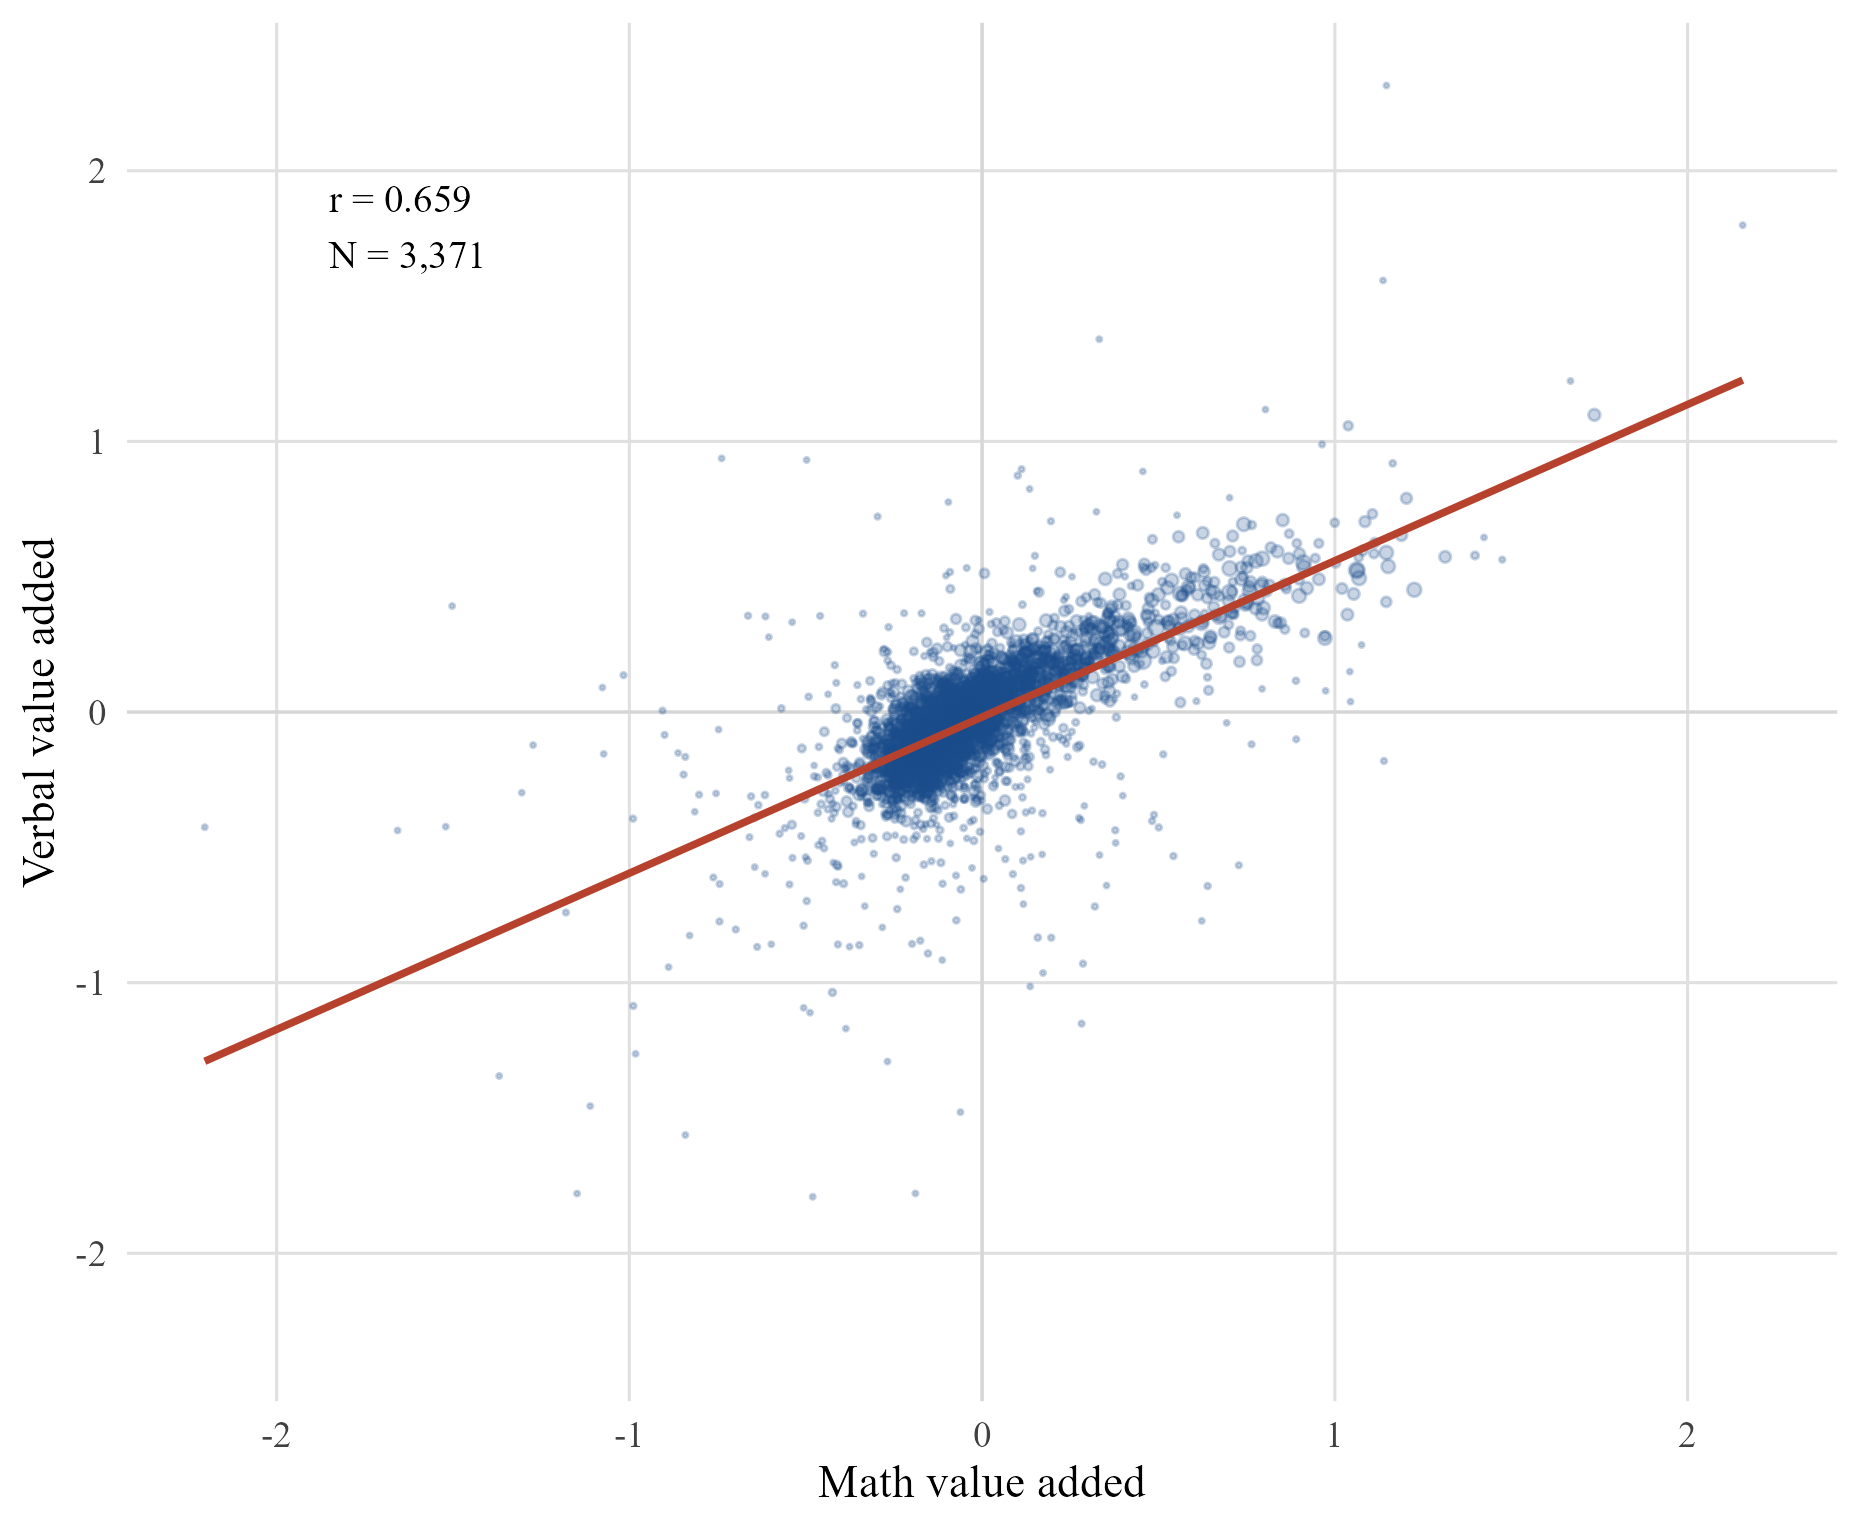
\includegraphics[width=.48\textwidth]{../../output/figures/results_section/math_language_va_correlation.png}%
}
\hfill
\subbottom[Math and high-premium-field value added\label{fig:math-highpay-va-correlation}]{%
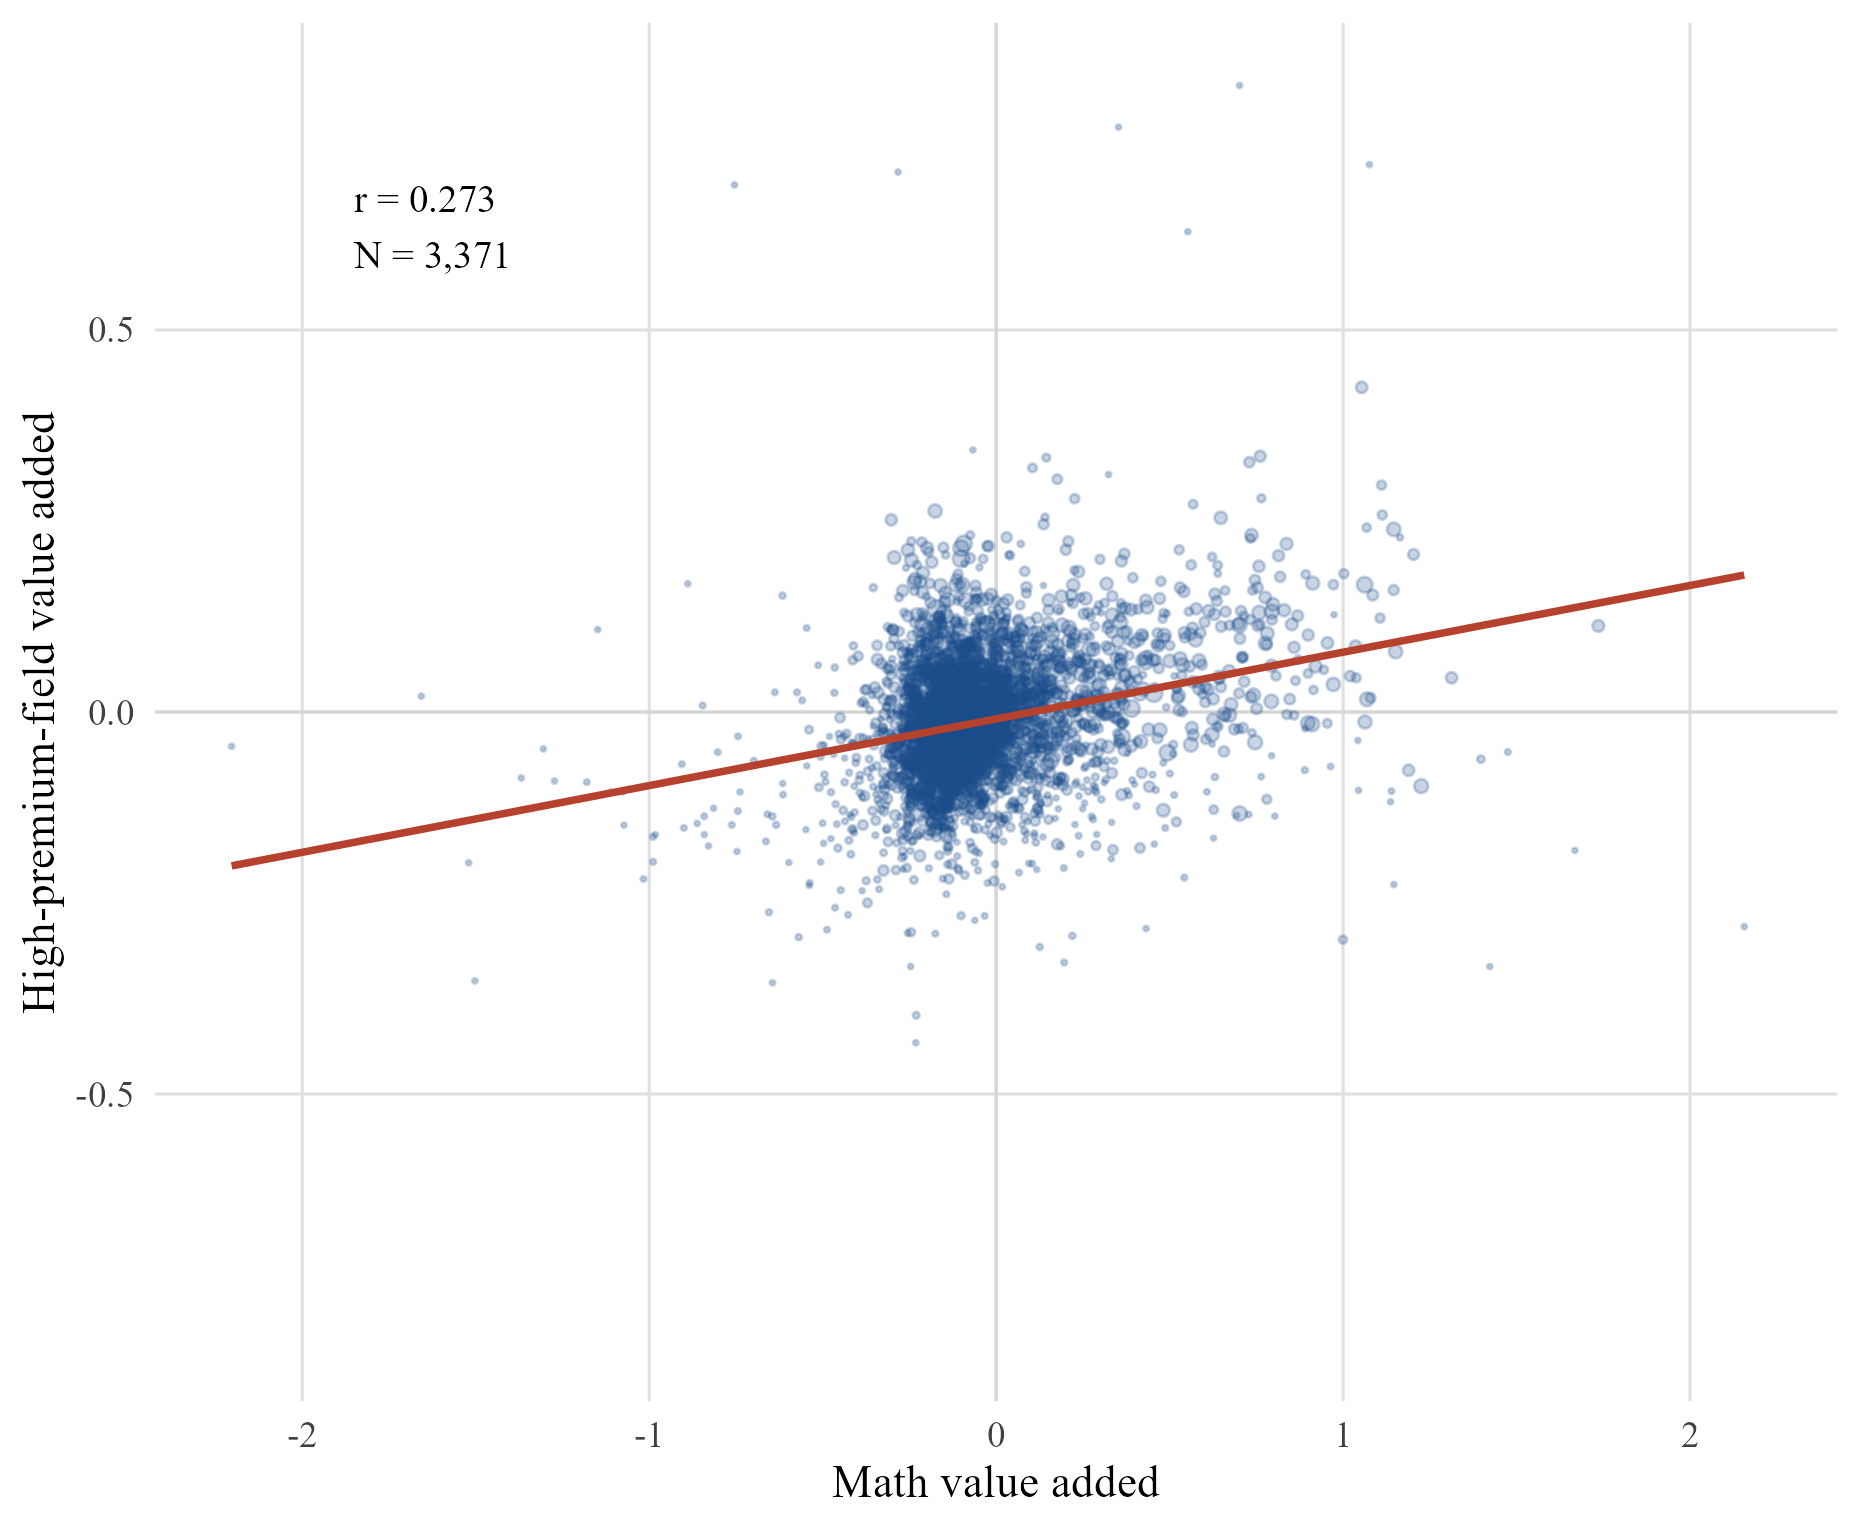
\includegraphics[width=.48\textwidth]{../../output/figures/results_section/math_highpay_va_correlation.png}%
}
\caption{Relationships between math, verbal, and high-premium-field observational value added}
\label{fig:va-correlation-panels}
\end{figure}
\FloatBarrier

I estimate a joint IV regression for log projected program income using the ordered EB value-added measures specified in equation~\ref{eq:ordered-va-iv}.
Each attended school value is instrumented with the corresponding first-round offered-school value, and the regression controls for the assignment-risk expected value of each dimension.

Table~\ref{tab:program-income-orthogonal-math-highinst-highpay} reports the estimates.
Math value added has a small and statistically insignificant coefficient of $-0.056$.
High-premium-institution value added net of math is positive, with an estimate of 0.286.
High-premium-field value added net of math and high-premium-institution value added is positive and precisely estimated, with a coefficient of 0.366.
These estimates are difficult to reconcile with a view in which math value added fully summarizes the school dimensions relevant for projected income.
Instead, high schools appear to have labor-market-relevant value-added dimensions that are not captured by achievement value added alone.
%The strongest evidence comes from the incremental high-premium-field dimension: schools that shift students toward high-premium fields also raise projected income after accounting for math and institution-choice value added.
%The raw joint horse race gives the same qualitative message, but the ordered version makes the incremental interpretation more transparent.

\begin{table}[!htbp]
\centering
\caption{Ordered IV horse race for log projected income}
\label{tab:program-income-orthogonal-math-highinst-highpay}
\begin{tabular}{lc}
\toprule
 & Log proj. income \\
\midrule
Math VA & -0.056 \\
 & (0.057) \\
High-premium-institution VA net of math & 0.286** \\
 & (0.143) \\
High-premium-field VA net of first two & 0.366*** \\
 & (0.096) \\
\midrule
N & 95,621 \\
\bottomrule
\end{tabular}
\par\medskip
\footnotesize
\begin{minipage}{\textwidth}
Notes: The dependent variable is log projected program income. The table reports an ordered horse-race IV. Math VA enters first; high-premium-institution VA is measured net of math VA; high-premium-field VA is measured net of the first two dimensions. This ordering is used to aid interpretation and does not make the coefficients structural returns to achievement, institutions, or fields. Attended-school values are instrumented with the corresponding first-round offered-school values, and the regression controls for the DA-probability expected value of each dimension, cohort, grade-4 SIMCE math and language, gender, and age. Heteroskedasticity-robust standard errors are reported in parentheses. $^{*}p<0.10$, $^{**}p<0.05$, $^{***}p<0.01$.
\end{minipage}
\end{table}


\FloatBarrier

\clearpage 
\section{Conclusion}

This paper asks whether high schools causally affect higher-education choices, and to what extent those effects are captured by observational value added.
I address this question by combining Chile's centralized school assignment system with linked administrative data.
I first estimate school value added for achievement and higher-education outcomes in a broad national panel, and then use lottery offers to ask whether schools that look better in observational value-added terms also produce larger causal effects.

The main estimates suggest meaningful pass-through.
The estimates are 0.884 for math, 0.885 for verbal achievement, 0.497 for high-premium-institution enrollment, 0.803 for high-premium-field enrollment, and 0.311 for log projected program income.
In practical terms, schools that observationally look better at raising achievement or higher-education outcomes also predict causal effects on those same outcomes, as I can confidently reject $\theta = 0$ in all dimensions of value added.
The results therefore show that the school assignment margin shifts later higher-education choices, not only test scores.

The heterogeneity results show that the relationship is mostly stable across students, with noticeable exceptions.
Relative to students in the middle quintile of baseline math achievement, math value added is substantially less predictive in the bottom quintile and marginally more predictive in the top quintile.
At the same time, both verbal and math achievement show noticeable gender differences in their forecast coefficients.
These differences may suggest some caution when considering achievement value-added disclosure policies, especially in terms of their efficacy and equity across groups.
However, the non-achievement results are remarkably stable, making the common-effects approximation more plausible for those dimensions.

%For verbal achievement and the three higher-education outcomes, none of the differences relative to the middle quintile is statistically significant.
%These results point to meaningful heterogeneity in math pass-through, rather than a common pattern across outcomes or the baseline achievement distribution.

Finally, I ask which dimensions of school value added predict gains in projected program income.
The ordered horse-race exercise enters math value added first, then high-premium-institution value added net of math, and finally high-premium-field value added net of the first two dimensions.
In this joint IV specification, math value added is small and statistically insignificant, while the two higher-education choice dimensions are positive and significant.
These results suggest that high schools differ along multiple dimensions in ways that are not captured by achievement alone.
In particular, schools affect higher-education decisions through dimensions not captured by math achievement, such as institution and field choice.
%The analysis does not determine whether these differences arise from counseling, information, expectations, peer norms, academic preparation, or other school practices.

These results show why achievement-based measures of school quality are incomplete.
As access to secondary and higher education expands, the consequences of schooling increasingly depend not only on learning and enrollment, but also on the decisions students make thereafter.
Accountability systems and school-choice policies centered on achievement may therefore overlook school effects that matter for the allocation of skills across fields, occupations, and sectors.

The results also qualify how higher-education choices should be interpreted.
Decisions not to continue to higher education, to avoid particular fields, or to attend lower-quality institutions are often interpreted as revealing stable preferences or privately optimal responses to expected returns.
Yet both expected returns and the options students perceive can be shaped by the information, expectations, academic preparation, and support they receive in high school.
A decision may therefore be privately optimal given beliefs and preparation that the high school helped produce, while still being causally affected by the school attended.
This possibility is especially important in settings where families have limited information about educational options and where access to counseling and other supports varies across schools.

%Future work should attempt to identify the specific channels that generate these effects and examine whether families value and respond to nontraditional measures of school value added.
%It should also study whether providing information on multiple dimensions of school quality changes school demand and later educational choices, and estimate the aggregate consequences of systematically ignoring these dimensions when students and funds are allocated across schools.

\clearpage
\printbibliography
\end{document}
